\subsection{复杂危险作业场景模拟及训练}

早在 20 世纪末,人们就已经认识到虚拟现实技术在仿真训练中的巨大作用。一篇 2001 年关于南非煤矿环境中利用虚拟现实进行安全训练的文章\endnote{Squelch A P. Virtual reality for mine safety training in South Africa[J]. Journal- South African Institute of Mining and Metallurgy, 2001, 101(4):209-216.}指出利用虚拟现实技术在特殊环境下进行安全训练的速度和可接受程度均高于使用传统图文或视频资料的对照组,说明了漫游行为在用户认知复杂环境中起到了不可或缺的作用。图\ref{fig:mine}即演示了一种突如其来的岩石垮塌的情形,需要被训练的工人根据情形作出操作来避免危险。

\begin{figure}[htp]
\centering
\fbox{
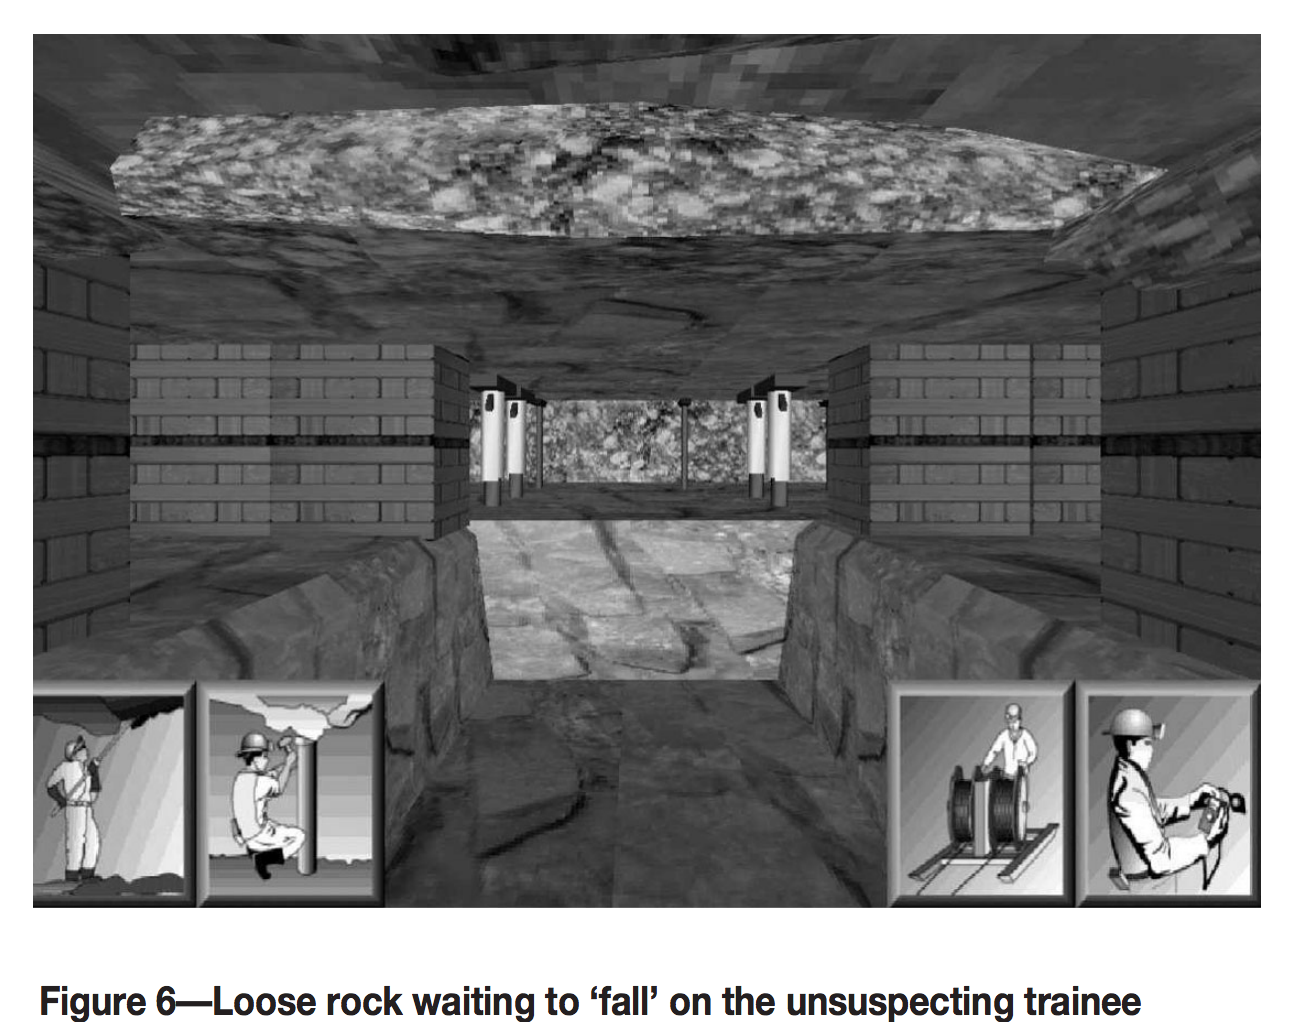
\includegraphics[width=.7\textwidth]{mine}
}
\caption{煤矿岩石垮塌模拟}
\label{fig:mine}
\end{figure}

虚拟现实技术还可被应用于航空航天训练、危险环境救援演练及其他人类无法安全、便捷进入的自然环境中,有效地拉近了使用者与模拟的真实环境间的认知距离,在保证安全的前提下高效完成训练任务。

\subsection{仿真虚拟环境}

另一种虚拟现实所应用的领域为建筑规划设计行业,因其所涉及的事物过于庞大,难以从普通的二维视图中体会其中的空间感,通过虚拟现实的技术则可以不必耗费大量精力搭建实物模型便能够身临其境般地感受建筑的尺度。

来自日本横滨国立大学教育学院的团队通过云计算 VR 系统帮助研究者快速搭建城市场景并实时查看、分享、交流与评估
\endnote{Zhang, Y., Shen, Z., Wang, K., Kobayashi, F., Lin, X. Cloud-based Virtual
Reality Integrated Automatic Presentation Script for Understanding Urban Design
Concepts in the Consensus Process: A Case Study of One Foundation Disaster Prevention
Park in China[J]. International Review for Spatial Planning and Sustainable Development,
5(1), 29-44. 2017.}。通过数字城市系统(如图\ref{fig:urban}),用户可以以自己想要的方式自主漫游整个场景。

\begin{figure}[htp]
\centering
\fbox{
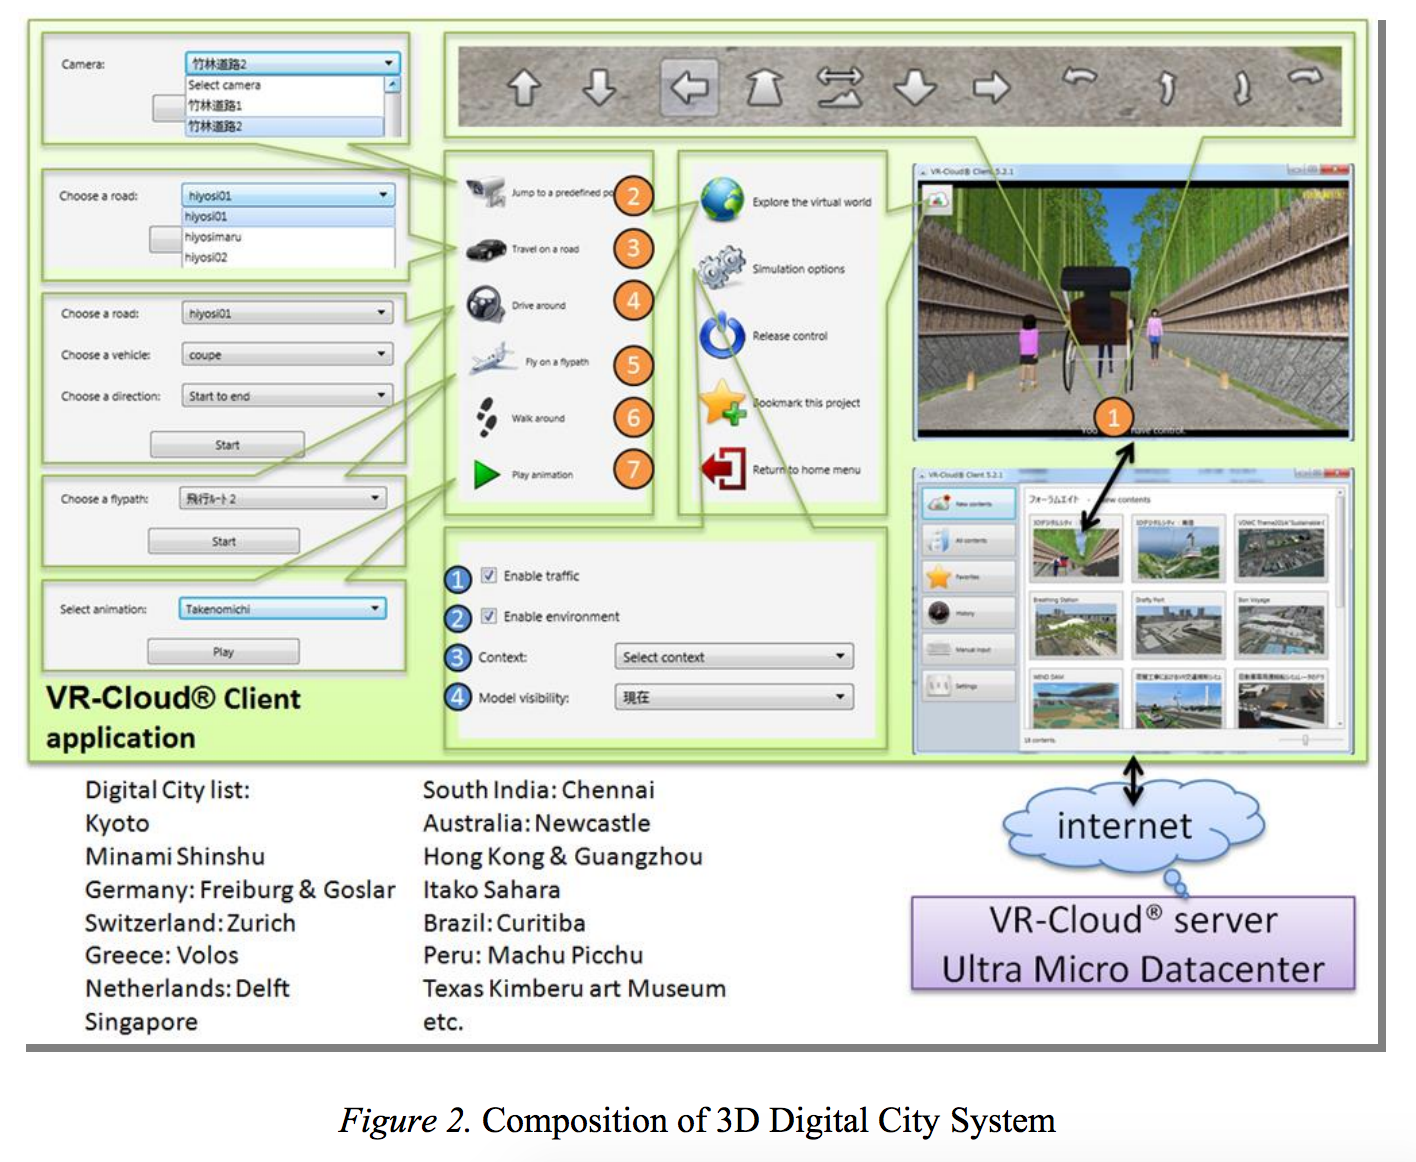
\includegraphics[width=.7\textwidth]{urban}
}
\caption{3D 数字城市系统}
\label{fig:urban}
\end{figure}

建筑信息模型(即 BIM)早已进入建筑工程项目的各个领域,全景漫游在技术和数据上几无障碍,且国内 BIM 技术也已较为成熟,充分利用全景漫游技术于建筑设计施工的方方面面将有利于设计者更直接地面对设计产物,提前发现设计中不完善的地方并加以改进。同时,将全景漫游的体验带给普通消费者,也有助于潜在购买者产生购买的欲望和动机。

\subsection{医疗康复}

医疗领域中虚拟现实技术的应用前景非常巨大,例如帮助因意外事故失去肢体或瘫痪的患者掌握使用假肢等。这些病患们的神经系统可以通过虚拟现实体验获得增强,他们能够在虚拟的环境内通过想象自己使用肢体进行运动、借由脑电波通过神经电位向计算机传递信号以操控虚拟环境内的肢体,在不断的反馈式训练过程中阶段性地磨合人与机器的灵敏程度,最终实现康复(见图\ref{fig:health})。相关专家称瘫痪的患者其实尚存在一些完好无损的神经组织,但因皮质和肌肉均未发射神经信号,这些神经将保持沉默数年。而利用虚拟现实的治疗将通过人机界面的训练重新唤醒这些神经,经过强化后将能够部分或完全地将大脑皮质运动区的信息传递到骨髓神经。

\begin{figure}[htp]
\centering
\fbox{
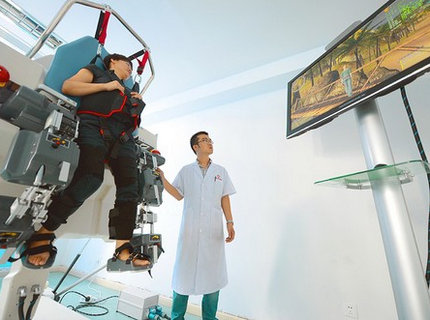
\includegraphics[width=.7\textwidth]{health}
}
\caption{瘫痪患者在进行治疗}
\label{fig:health}
\end{figure}

同时也有相关团队期望利用虚拟现实技术对患有自闭症的儿童进行适应性训练,在对超过 100 名智力正常的学龄儿童进行四面全沉浸式 CAVE VR 训练实验后,被试儿童们在情绪认知、情感表达及社交等领域表现出了显著的提升\endnote{Ip H H S, Wong S W L, Chan D F Y, et al. Virtual Reality Enabled Training for Social Adaptation in Inclusive Education Settings for School-Aged Children with Autism Spectrum Disorder (ASD)[M]// Blended Learning: Aligning Theory with Practices. Springer International Publishing, 2016.}。
